\chapter{Training process}

\section[Exploitation of spatial symmetries]{Exploitation of spatial symmetries \hfill \small \normalfont\textit{by Matthias Hericks}}



In an early stage of the project, we noticed that the environment exhibits multiple spatial symmetries and though about how this can be exploited, when training an agent. Loosely speaking, if an agent knows how to act in a particular state $s$, this information can be used by the agent to act in the seven different states, which arise as symmetric transformations - flips / rotations / transposition - of the state $s$, given that its actions are transformed accordingly.
% TODO: http://www.cs.cmu.edu/~maz/publications/symmetry7.pdf
% TODO: https://alexandria.physik3.uni-goettingen.de/PDF/agostinicelaya2009
A search in relevant literature revealed that \ref{} identifies these symmetries as symmetries with \emph{adherence to an equivalence relation}. Moreover, \ref{} describes two multiple possibilities to exploit these symmetries in the training process of an agent.

\vspace{10pt}
\begin{center}
\begin{minipage}{\linewidth}
\includegraphics[scale=0.2]{graphics/symmetries.png}
\captionof{figure}{Visualisation of 8 states in the same equivalence class w.r.t. $\sim_{\text{sym}}$.}
\end{minipage}
\end{center}
\vspace{10pt}

The key idea is to define an equivalence relation $\sim_\text{sym}$ on the set of all states, such that $s \sim_\text{sym} s'$ if and only if there exists a sequence of symmetric transformations, which maps $s$ to $s'$. For every equivalence class under this relation, we fix one particular state in this class as the \emph{candidate} state. Therefore, for each state $s$ there exists a candidate state $s_\text{can}$, such that symmetric transformations can be used to transform $s$ to $s_\text{can}$. Instead of training on all possible states, the agent now merely trains on the candidate states. After each state transition the new state is transformed to the corresponding candidate step in a preprocessing step before presenting it to the agents learning method. Moreover, a special map is computed, which maps the action of the agent in the candidate state to the associated action in the original state of the environment in a postprocessing step. By doing so, we effectively divide the number of states which the agent encounters by 8, as seen in the graphic on the previous page. \\

We conducted a simulation study, comparing the convergence of a simple coin-collecting agent with varying exploitation of symmetries and obtained similar result as the ones by \ref{...} (compare \ref{...})

\section[Feature design]{Feature design \hfill \small \normalfont\textit{by Mika Rother}} \label{sec:feature_design}
\subsection{Simple features}
First of all, a linear model requires good feature design. Since many features cannot be represented by such a model, the return values of a feature had to be either 1 or 0. Accordingly, it is not possible to create a \textit{numpy array} that indicates for all bombs on the field how long a bomb needs to explode. In such a case, one would logically need an array for each time step of a bomb in a linear model that indicates whether a bomb will explode after as many time steps.
\\

Accordingly, the first step was to design simple features that could be used to analyse the agent's behaviour and achieve initial training results. At the same time, it was also important that the features did not define a desired behaviour too precisely, so that the agent still had to learn to behave well itself. 
\\

So the work started with designing features that would teach the agent on a field without crates and only with coins to collect these coins as efficiently as possible.

\subsubsection*{Coins per quarter}
The first feature that was developed was very simple: coins per quarter. The idea of this feature was based on giving the agent four features, where each of the features was for one of the possible moves, (where \texttt{'WAIT'} and \texttt{'BOMB'} were taken out as possible actions for this part, because it wouldn't make sense to place bombs or wait on a board without crates). The playing field was accordingly divided into top left, top right, bottom left and bottom right. Then the sum of the coins in each of these quarters was added up and given to the agent, so that he was always informed in which part of the field the most coins could be collected. 
\\

Training with these features alone led to some problems, of course. On the one hand, it could happen that a change of position led to a situation where suddenly the most coins were in a different quarter than in the step before. This often resulted in a back and forth movement, which is of course very inefficient. On the other hand, the agent often passed by nearby coins on the way to the quarter with the most coins. To fix this problem, we gave the agent more features.

\subsubsection*{Relative environment of the agent}
Since the agent had not been aware of its immediate surroundings so far, \textit{relative maps} were created to tell it which objects are in its immediate neighbourhood. Since only \textit{walls} and \textit{coins} were on the field at this point, maps were first created for these two objects. These then had the following format:
\vspace{0.1cm}
\lstinputlisting[caption=]{listings/rel_wall_coin_map.py}
\vspace{0.1cm}
So both were maps of size $31\times 31$. The idea of these maps was that the agent is always in the centre (\texttt{pos = [15,15]}) and sees the environment from his point of view. This had to include a total of 31 fields on both axes so that the agent also had a complete map available in the corners of the field.
\\

It is easy to calculate that $31\times 31$ entries for two maps lead to an extremely large number of features, since each field has either the value 0 or 1, depending on whether the object to be examined is located on this field or not. Therefore, and because primarily the immediate environment of the agent is interesting, another variable was introduced, the \texttt{NUM\_LOOK\_AROUND}. If, for example, the value 3 was chosen for this variable, the agent only got informations about his environment with radius 3, i.e. three fields in each direction from the agent and thus a $7\times 7$ array for the relative maps. With the help of these features, considerable progress could already be made, even if the road to perfection was still a long one.

\subsubsection{Escape death features}
So, since the agent was able to collect coins in an acceptable time, the next step on the list was to move on to crates. Now the agent first had to learn to plant bombs to destroy crates without blowing himself up, and then collect the coins that appeared in the explosion. This task proved to be much more difficult, as the agent still had to earn as many coins as possible without blowing himself up. 

\subsubsection*{Get all safe tiles}
The first step was to find all the fields that could turn out to be unsafe. For this the function \texttt{get\_unsafe\_tiles()} was written, with the help of which one could check which fields in the periphery of a bomb were dangerous, i.e. on which fields the agent would not be allowed to stay without diying if the bomb exploded. This function was then passed the \texttt{field} and the \texttt{bombs} on each turn, which could be imported from the current \texttt{game\_state}.
\\

Furthermore the function \texttt{get\_reachable\_tiles()} was created. This function was passed the current position of the agent (\texttt{pos}), the number of steps the agent can still walk until the bomb explodes (\texttt{num\_steps}) and again the current playing field (\texttt{field}). Using this data, the function could then determine which fields could still be entered in a given number of steps. \vspace{0.2cm}

These two functions were now used to find all fields that can still be entered in a given number of time steps without dying. This resulted in the following function:
\vspace{0.1cm}
\lstinputlisting[caption=]{listings/get_reachable_safe_tiles.py}
\vspace{0.1cm}
With the help of this function it was now possible to teach the agent not to enter fields that led to a certain death. Because the function \texttt{get\_reachable\_safe\_tiles} returns all positions, which an agent can still enter without dying.


\subsubsection*{Get safe death features}
However, in order to be able to represent the whole thing as a feature in a linear model, of course only binary values (0 and 1) may be returned, so that training can be done in the correct way. Accordingly, a new function was created, which creates a numpy array with five entries (for the actions: \texttt{'UP', 'DOWN', 'LEFT', 'RIGHT'} and \texttt{'WAIT'} and depending on which action is feasible without dying, has a 0 or 1 in the respective entry.  
\\

For example, if the agent can only go up to avoid dying, the new function would return the following:
\vspace{0.1cm}
\begin{lstlisting}[language=python, keywordstyle=\color{black}]
  ret = ([0,1,1,1,1])    # (['UP','DOWN','LEFT','RIGHT','WAIT'])
\end{lstlisting}
\vspace{0.1cm}
The function that creates this output is called \texttt{get\_safe\_death\_features}. Thus, in addition to the possibility of collecting coins, a list of features was now given to help the agent understand which fields it would be better to stay away from in order to avoid death.
\\

Up to this point, the agent was simply trained to avoid fields that could end in his death. However, he was not explicitly told not to commit suicide. For a behavior that should be avoided in any case that the agent blows himself up by his own bombs. For example, it should be made clear to him at the beginning of the game that he must not die by planting his own bombs. This idea served mainly to ensure that the first action is not \texttt{'BOMB'}, since that usually ends in certain death. Therefore, another feature \texttt{is\_bomb\_suicide()} was developed, which returns whether a bomb planted by the agent led to his death.

\subsubsection*{Relative maps for escape death features}
To round off the whole thing, relative maps for crates were generated, which were used to pass the crates in the immediate vicinity to the agent for training. The aim here was, of course, that the agent finds the way to neighboring crates as quickly as possible and does not have to search for so long.
\\

As mentioned at the beginning of this chapter, in order to have all the time steps of all bombs and where they do damage, it would be necessary to create a relative map for each time step of a bomb. Since it would then be necessary to create four different maps, corresponding features were written, but rarely used for training, since it would then have been much more difficult to find good weights. And one of the goals of reinforcement learning is to train the agent with well-chosen rewards and not with a large selection of features.

\subsection{Shortest paths}
Now the point had come where our agent was performing his tasks to some extent, but not yet very efficiently. Therefore it was necessary to give him not only his environment, but actually the way he has to go, if he wants to find the next coin, for example. Since it is often important to know not only the way to the next coin, but also to the next crate or opponent, the function that calculates this shortest path had to be valid for several objects.
\\

The first approch that was taken was a simple \textsl{breadth-first-search} algorithm that treats the game board like a maze.

\subsubsection*{BFS in a maze}
In order to be able to represent the playing field as a labyrinth, a distinction had to be made in the first step between accessible fields and walls. Logically, fields with a wall or a crate were displayed as walls, the rest were displyed as free fields. This was then stored in an array (\texttt{free\_tiles}) that has the same shape as the game board. 
\\

Based on this array, it was then checked if the agent has the possibility to reach its target. The parameters \texttt{free\_tiles}, \texttt{start} and \texttt{target} were passed to the function \texttt{shortest\_path()}. Here, the positions \texttt{start} and \texttt{target} represent the position of the agent and the position of its target. A maze was then created, looking in each iteration to see which points could be reached with how many steps. The search algorithm that was used for this process was \textit{breadth-first-search} (BFS). If the target position was reached, the search ended and the path was reconstructed. If no path could be found, the position of the agent was returned. 
\\

Although the shortest path could be calculated using this function, there was a major problem: the maze was recalculated for each step, which took about two seconds. That doesn't sound like much, but if one wants to train several workouts with at least 100 laps, then that was definitely too much.

\subsubsection*{A* search}
An algorithm for finding the shortest path is the A* search algorithm. This is a generalization and extension of Dijkstra's algorithm, although Dijkstra's algorithm can also be reduced to the A* search algorithm. Now a new class has to be introduced to perform A* search:
\vspace{0.1cm}
\lstinputlisting[caption=]{listings/class_nodes.py}
\vspace{0.1cm}
A node is thus initialized with a parent, a position and values $f,g$ and $h$. The A* search algorithm always examines the nodes first that are the most probable to lead to the goal. For this, the values for $f,g$ and $h$ are required. If $x$ is a node, the following relation holds:
\begin{align}
f(x) = g(x) + h(x)
\end{align}
In this context, $f(x)$ is the estimated distance from the starting node to node $x$, $g(x)$ denotes the previous cost from the starting node, and $h(x)$ is a heuristic that estimates how far it is from the current node to node $x$.
\\
 
Let $u$ and $v$ be two nodes and let $v$ be the target node. Then the heuristic that was used in our A* search algorithm is given by
\begin{align*}
h(u) = 2\cdot(u[x] - v[x]) + 2\cdot(u[y]-v[y])
\end{align*}
where $x$ and $y$ describe the coordinates of the game board. The choice of the heuristic is only a small detail, which can be improved, but since later only the nearest coins are considered, this was not necessary here. Nevertheless, an alternative evaluation function is given here, which Xiang Liu et al. tested in [\ref{..}] for different mazes:
% TODO: BibTex einfügen: https://www.researchgate.net/publication/238009053_A_comparative_study_of_A-star_algorithms_for_search_and_rescue_in_perfect_maze
\begin{align*}
f(x) = g(x)+h(x)+h(y)
\end{align*}
where $y$ is the parent node of $x$. The is equal to the definition of the evaluation funtion defined in Eq. (2.1).
\\

The A* search algorithm then creates two lists with the open nodes and the closed nodes. Then, starting from the starting node, the neighbors are traversed and whenever a node is found that has not yet been added to the closed nodes, a check is made to see if it is already among the open nodes. If not, it will be added and its $g$ value will be increased by one compared to the node from which it was reached. If the node is already in the list of open nodes, it is checked if the new $g$ value is smaller than the previous one. If it is, the entry is renewed. This also ensures that the parent node is always initialized with the predecessor node from which it is quickest to get to the current node.
\\

If a shortest path to a position is found using this algorithm, this position is returned. If not, the position of the agent is returned instead. It has been shown that this algorithm is much faster than the maze-based BFS algorithm. However, the structure of the nodes has not yet been fully exploited, so the $f$,$g$, and $h$ values have not yet been well accounted for.

\subsubsection*{A* search with priority queue}
To get the last bit of performance out of the algorithm, it was necessary to store the open nodes list as a priority queue, where the priority in this case is determined by the $f$ value of a node. The Python module \texttt{heapq} was then used for this, which provides basics for efficient data structures. This finally allowed a satisfactory runtime to be achieved, especially since later only the objects nearest to the agent were considered. And accordingly not all objects had to be traversed.

\subsubsection*{Find shortest path to specific objects}
Once an efficient algorithm was available that could calculate the shortest path, the next step was to calculate only the shortest path to the objects of a class that were really close. Given the list of positions of all crates, one wanted to include only the relatively close crates in the calculation, since for example the amount of crates with a \texttt{CRATE\_DENSITY} of $0.7$ would be very large and a calculation of the shortest paths to all would cost too much performance. 
\\

Therefore, a function was written that is passed the list of objects, let's take coins as an example, and then finds the shortest Euclidean distance between the agent and the nearest coin using the following nesting numpy function (\texttt{best\_dist}):
\vspace{0.1cm}
\lstinputlisting[caption=]{listings/best_dist.py}
\vspace{0.1cm}
But since the coin with the shortest Euclidean distance to the agent is not necessarily the one with the shortest path, one could still extend the \texttt{best\_dist} with an \texttt{offset} so that the shortest path from the agent to all coins in its neighborhood with radius $R$:
\begin{align*}
R = \texttt{best\_dist} + \texttt{offset}
\end{align*}
was calculated.
\\

The shortest path functions were then used to find the shortest paths to the next coin and to the next crate. When the shortest path function was tested with the agent collecting only coins, the results were much better than with the previous features. The idea behind using this feature for the crates as well was based on the observation that when training the agent with crates and bombs, he often did not move to other crates to destroy them. By training the agent to take the shortest path to crates, much better results could be achieved.

\subsection{All features combined}

\subsubsection*{Last small feature}
Since the agent had been taught during the training with all the features described so far that he had to plant bombs to destroy crates, i.e. received a positive reward for it, unfortunately the problem occurred that whenever he could plant a bomb, he also placed one, even if no crates were destroyed by it. Therefore, another feature was needed that simply indicates whether the agent is standing next to a crate or not, with the idea that this would teach the agent to place bombs more often if it destroyed crates.

\subsubsection*{Play and train with all features}
Based on all the features described so far, the agent could be trained to be capable of destroying crates and collecting the coins that appeared without dying. However, this did not always succeed and even when it did, sometimes more sometimes less well (more on this below). 

\subsection[Genetic algorithm for feature extraction]{Genetic algorithm for feature extraction \hfill \small \normalfont\textit{by Matthias Hericks}}
At some point it was evident, that we spend more and more time on the construction of increasingly complex features. Since this is a machine learning project, we looked for ways to overcome this problem and came up with two possible directions:
\begin{enumerate}
	\item Choosing a different (nonlinear) approximation function, like deep neural networks, decision trees or regression ensembles with gradient boosting.
	\item Finding a way to learn good features (automated feature extraction).
\end{enumerate}
 
We knew from extensive communication with other groups, which opted for option 1, that a change in the approximation function would not be straight-forward. Many more complex function approximators rely on off-policy batch gradient-descent updates and on-policy $n$-step Sarsa and Sarsa($\lambda$) learning algorithms are not applicable at scale. Our initial idea was to implement PCA with training data from the rule based agent, since it is reasonable that the same features resulting in a good performance of the rule based agents might help our agent. A detailed discussion with the group of Fabian Kneissl, revealed that PCA was not applicable here. To explore some new grounds, we read a lot about genetic algorithms for feature selection and extraction with \cite{cha2008}, \cite{nguyen2011} and \cite{li2005} being our primary sources. \\

The key idea, was to rewrite one of our ordinary linear agents, such that its training process depends on a a list of binary expression trees, which each represents a boolean expression. We will call such an agent a \emph{genetic agent}. By default we provide the genetic agent with all of the complex features mentioned above as well as a high number of simple features, e.g. maps representing the agents relative environment up to four tiles in each direction. We will denote this high-dimensional feature vector of a state $s$ by $x(s)$ and call $x(\cdot)$ the \emph{raw features}. All of the boolean expressions represented by the trees, take fixed components of the raw feature vector as input and therefore represent composite features depending on one or multiple raw features. Instead of using all of the raw features for the linear function approximation of the action-value function $q$, the genetic agent now learns with its composite functions. Therefore, the effective number is of features used in the linear regression is no longer the (possibly large) dimension of $x(\cdot)$, but merely the length of the agents list of binary expression trees. \\

\textbf{The problem with simple features.} \\

To give a concrete example, lets assume that the raw feature vector $x(s)$ contains one-hot encoding of the agents surroundings. In a linear model this is only of limited benefit for the agent, since many important situations can not be described well by such a model. If a bomb is one tile above and two tiles to the right from the agent, it is quite possible, that the linear agent will learn to avoid the action \texttt{UP}, since in some situations such a bomb might have killed it. However, in a linear model the agent will shy away from the action \texttt{UP}, even if there is a wall one block above and one block to the right of him, which would block the bomb. If he still chooses the action \texttt{UP}, it is quite possible that the wall to the top right of him adds positive value to the estimation of the \texttt{UP} action. However, this is not desirable if the tile above the agent is blocked. \\

Composite features might fix this problem, by introducing features like \texttt{is tile above free} \texttt{AND} \texttt{(is no bomb in the row above OR will a wall block such a bomb)}, \linebreak where most of the operands are itself composite expressions. Therefore, the aim is to find automatically construct binary expression trees, which represent good features. \pagebreak 

For this complex task, we introduced a genetic algorithm following the following process for feature extraction.

\begin{minipage}{\linewidth}
\begin{center}
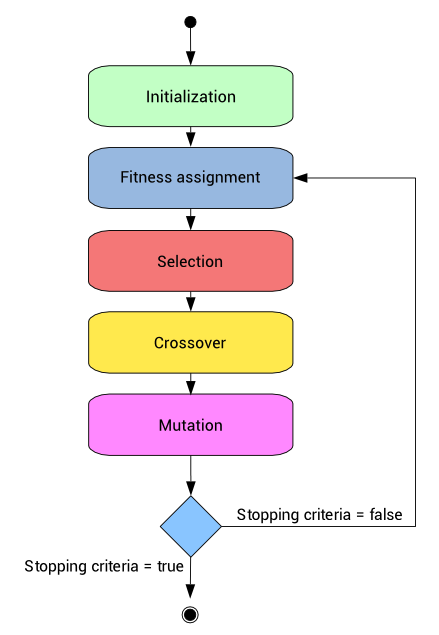
\includegraphics[scale=0.5]{graphics/genetic_algorithm.png}
\captionof{figure}{Modified feature extraction process from \cite{neural_designer}.}
\end{center}
\end{minipage}
\vspace{10pt}

An external script, initializes multiple lists of binary expression trees at random. We will call this set of lists the \emph{population} and one list of binary expression trees an \emph{individual}. Then for each of these individuals the fitness of the associated genetic agent is evaluated by training a linear agent with the corresponding composite features and measuring some kind of performance, e.g. average reward over the last 50 training episodes. After this is done for all the individuals, the best performing agents were selected as \emph{the offspring} and cloned to create a new population. Moreover, on some of the clones mutation and crossover operations were performed. Mutation operations mutate some of the binary trees of an individual at random. Crossover operations take two individuals and exchange whole trees or subtrees. This resulting group of individuals is called the \emph{next generation}. The process is now iterated with the next generation as starting population. Throughout this process, the average performance of the individuals in the population are tracked, which hopefully increases. \\

For the implementation, we used the \texttt{DEAP} \emph{"Distributed evolutionary algorithms in python"} library, which gave us a lot of flexibility and even implemented some standard mutation and crossover operations on binary expressions trees. Using this method, we were able to construct good features in toy examples. One example being the selection of valid game-related features in a raw feature set with many random features (a feature returning 0 or 1 at random). Moreover, the genetic algorithm was able to find solutions to the simple feature problem mentioned above. \\

Unfortunately, there are still multiple flaws with this feature extraction algorithm.
\begin{itemize}
	\item For every new generation, the fitness of each new individual in the population has to be evaluated by training an agent. Since typically many generations are necessary to construct a good features, e.g. a good population, this easily results in long runtimes. 
	\item The genetic algorithm itself introduces a variety of hyperparamters, the primary ones being the population size, the mutation probability, the crossover propbability and the number of generations. Moreover, the concrete choice of mutation and crossover algorithms determines the failure and success of the algorithm. 
\end{itemize}
We tried to use as many heuristics and guidelines mentioned in the sources mentioned above, but in the end the deadline forced us to use our handcrafted features together with a few compound features motivated by the genetic algorithm. Still, the results in toy examples look promising and we are eager to learn more about genetic algorithms for feature extraction in the future. 





\section[Rewards and fine tuning]{Rewards and fine tuning \hfill \small \normalfont\textit{by Mika Rother}}
The first part of this section is about the different rewards we gave to the agent for different events. This part is further divided into a rewards available through regular events, i.e. for events that have already been defined from the beginning in \texttt{event.py}, and rewards based on custom events.

\subsection{Rewards based on regular events}
At the beginning, when the agent was only supposed to collect coins, we only needed a reward that would reward him for collecting a coin. Afterwards, when we wanted to teach the agent to plant bombs to destroy crates, the awarding of rewards became much more complicated. In order to train successfully, we had to teach the agent several things to instill the correct behavior. The following points had to be checked off:
\begin{itemize}
\item[•] The agent must be able to plant bombs to destroy crates
\item[•] The agent in any case is not allowed to blow himself up
\item[•] The agent must continue to collect the coins
\item[•] The agent should not perform too many invalid actions
\item[•] The agent should try to play fast and play efficient
\end{itemize}
To accomplish all these points, a certain amount of subtlety was required to set the rewards correctly. For example, if a parameter was changed too much, an undesirable behavior often emerged (more on this below). Here is an overview of the rewards we have used up to this point:

\begin{table}[h!]
\centering
\begin{tabular}{|| l | l||} 
 \hline
 Rewards &  Range of values\\ [0.5ex] 
 \hline\hline
  \texttt{CONSTANT\_REWARD} & $[-1,-0.1]$  \\[0.5ex] 
  \texttt{e.COIN\_COLLECTED} & $[5, 15]$ \\ [0.5ex] 
  \texttt{e.KILLED\_SELF} & $[-50 , -15]$ \\[0.5ex] 
  \texttt{e.CRATE\_DESTROYED} & $[2, 5]$ \\[0.5ex] 
  \texttt{e.INVALID\_ACTION} & $[-0.5,-0.1]$  \\[0.5ex] 
  \texttt{e.BOMB\_DROPPED} & $[-1, 2]$   \\ [1ex] 
 \hline
\end{tabular}
\end{table}

Two things in particular are noticeable here: 
\begin{itemize}
\item[1.] The range of \texttt{e.KILLED\_SELF} is quite large relative to the other rewards. This is because we have done a lot of testing on what happens when the agent is heavily punished for a suicide, and what happens when he is not punished so much for it. The latter might motivate him to plant more bombs, which is in principle a desired behavior.
\item[2.] We actually had training sessions where we gave the agent a negative reward for planting bombs, as well as rounds where we rewarded him for doing so. This is because we wanted to teach the agent to plant bombs only if they lead to the destruction of crates. In this case we increased the reward for \texttt{e.CRATE\_DESTROYED}.
\end{itemize}
We also used a negative constant reward, so the agent doesn't wait the whole game.

\subsection{Rewards based on custom events}
The problem caused by the second point was the following: As soon as the agent was given a reward for $\texttt{e.BOMB\_DROPPED} < 0$, it developed the behavior of only waiting, (or, if it was also given a negative reward for waiting, only making \texttt{LEFT}-\texttt{RIGHT} or \texttt{UP}-\texttt{DOWN} movements). So it was not an option to give him a negative reward directly for bombing.
\\

However, since we wanted to continue to make him more likely to plant bombs that also destroy crates, we developed our own events:
\vspace{0.1cm}
% \lstinputlisting[caption=]{listings/custom_events.py}
\vspace{0.1cm}
Now let's explain the sense of them:
\begin{itemize}
\item[•] \texttt{CRATE\_DESTROYING\_BOMB\_DROPPED}. As already mentioned, this is the event that should develop the behavior of destroying crates with dropping bombs. 
\item[•] \texttt{BOMB\_DROPPED\_NO\_CRATE\_DESTROYED}. This reward, on the other hand, should have exactly the opposite effect. For this event the agent should get a negative reward, because here the planting of a bomb does not cause the destruction of crates.
\end{itemize}
For these two custom events we could now also give rewards without rewarding the agent just for planting bombs. However, we still gave a reward for the event \texttt{e.CRATE\_DESTROYED} because we noticed that we can't set \texttt{CRATE\_DESTROYING\_BOMB\_DROPPED} too high without making the agent lay too many bombs again, thus simplifying fine tuning.
\\

Finally, here is the final overview of the rewards we used to train the agent:

\begin{table}[h!]
\centering
\begin{tabular}{|| l | l ||} 
 \hline
 Rewards &  Range of values\\ [0.5ex] 
 \hline\hline
  \texttt{CONSTANT\_REWARD} & $[-1,-0.1]$  \\[0.5ex] 
  \texttt{e.COIN\_COLLECTED} & $[5, 15]$ \\ [0.5ex] 
  \texttt{e.KILLED\_SELF} & $[-35 , -15]$ \\[0.5ex] 
  \texttt{e.CRATE\_DESTROYED} & $[2, 4]$ \\[0.5ex] 
  \texttt{e.INVALID\_ACTION} & $[-0.5,-0.1]$  \\[0.5ex] 
  \texttt{CRATE\_DESTROYING\_BOMB\_DROPPED} & $[2,7]$  \\[0.5ex] 
  \texttt{BOMB\_DROPPED\_NO\_CRATE\_DESTROYED} & $[-2,-0.5]$  \\[1ex] 
 \hline
\end{tabular}
\end{table}

With this set of events, training was further simplified. Unfortunately, it turned out that some behavior patterns were difficult to avoid and occurred again and again when testing the agent. For example, if the agent was standing right next to a crate and there were coins on the field at the same moment, the agent got into the habit of waiting if it had to increase the Euclidean distance to the next coin first, i.e. move away from the coin first to reach it.

\subsection{Fine tuning of other parameters}
The values that could be assigned to the various rewards were not the only changeable parameters that could be fine-tuned. We tested different values for various types of parameters from time to time in order to achieve the best possible training results. In the following, these various parameters are described and their variation is briefly explained. (The exact results for the important points can be read in Experimental results).

\subsubsection*{Variying hyper parameters}
The hyper parameters of the training were the \textit{learning rate} ($\alpha$) and the \textit{discount factor}. Based on the book of Sutton [\ref{..}] and of our simulation studies we learned that the following realtion leads to good results:
\begin{align*}
\alpha \times \texttt{NUM\_FEATURES} \approx \text{const.}
\end{align*}
So we tried to choose $\alpha$ so that this realtion is approximately kept. For the discount factor we achieved good results, when choosing 
\begin{align*}
\texttt{DISCOUNT\_FACTOR} \sim 0.85 \pm 0.1
\end{align*}

\subsubsection*{Variying policy type parameters}
During the project we used two different types of policies as explained in \ref{..}. In most cases the randomness was reduced with increasing number of training iterations. This yielded good results for both $\epsilon$-greedy and the softmax policy.

\subsubsection*{Variying parameters of update algorithms}
In total, we used three different update algorithms:
\begin{itemize}
\item[•] Sarsa,
\item[•] $n$-step-Sarsa and
\item[•] Sarsa($\lambda$),
\end{itemize}
where Sarsa is the same as $n$-step-Sarsa with $n=1$. For $n$-step-Sarsa, we obtained good results by choosing $n$ between 3 and 6. For Sarsa($\lambda$), we could choose the parameter $\lambda$ between 0.7 and 0.95 to get good results.












